\newpage
\section{INTRODUCTION}
\pagenumbering{arabic}
\setcounter{page}{1}
\enlargethispage{\baselineskip}

%%%%%%%%%%%%%%%%%%%%%%%%%%%%%%%%%%%%%%%%%%%%%%%%%%%%%%%%%%%%%%%%%%%%%%%%%%%%%%%%%%%%%%%%
%%%%%%%%%%%%%%%%%%%%%%%%%%%%%%%%%%%%%%%%%%%%%%%%%%%%%%%%%%%%%%%%%%%%%%%%%%%%%%%%%%%%%%%%
Most of the newly discovered active pharmaceutical ingredients (APIs) are poorly water-soluble in crystalline forms, which limit their bioavailability - dissolution and then their distribution through the organism. This fact limits their wider oral use as a solid drug in medical treatment. Nowadays, the techniques of combinatorial chemistry and high throughput screening have led to a sharp rise in the quantity of non-soluble API molecules, so the oral administration of poorly soluble drugs became the biggest challenge for formulation scientists in the pharmaceutical industry. \cite{leuner_improving_2000} There are different strategies to overcome this issue such as cocrystal formation \cite{batisai_solubility_2021}, convertion of API to its salt \cite{huang_impact_2004} or using solid dispersion. \cite{srinarong_improved_2011} 

In 1961, Sekiguchi and Obi provided the earliest account of so-called first generation solid dispersion, when they discovered that the creation of eutectic mixtures enhances the rate of drug release and bioavailibility. The first generation solid dispersion were built from crystalline carriers such as urea or sugars forming crystalline solid dispersions. The second generation solid dispersion was replacing crystalline carriers by amorphous carriers such as polymers, forming amorphous product, in which crystalline API is dissolved. There exist also third generation of solid dispersion using surfactant carrier or combination of amorphous polymers and surfactants.~\cite{vasconcelos_solid_2007}

Our aim is to overcome the poor solubility by using amorphous solid phases of APIs and to avert the rearrangement of molecules into a crystal lattice. However, crystalline forms of APIs are advantageous due to their better stability during long-term storage and better predictions of changes at the molecular level under defined conditions, using crystalline forms limit the bioavailibility. \cite{caron_comparison_2011} The better solubility of APIs in amorphous forms originates from a higher Gibbs energy of the amorphous form in comparison with the crystalline forms. During processing, storage, and after contact with water or humidity, the thermodynamically metastable amorphous forms tend to crystallise. Solid mixtures of API and excipients (e.g. polymeric excipients) create amorphous solid dispersions (ASD), and offer a way to inhibit crystallisation of the API before and after oral administration of the dose. \cite{prudic_thermodynamic_2014}

The addition of an excipient to an amorphous API can generally have a twofold effect on the rate of solid-state crystallisation, affecting both thermodynamic and kinetic aspects. Thermodynamically, it reduces the Gibbs energy due to strong intermolecular interactions between API and its excipient, as well as it increases kinetic barriers to recrystallisation. On the atomic scale of individual interactions, hydrogen bonding has the biggest contribution. \cite{newman_what_2022}

\section{Studied compounds}
    \subsection{Polylactic acid}
    Polylactic acid (PLA) was chosen as a biocompatible polymer excipient.  PLA is a biodegradable polymer formed by polymerisation of lactic acid. The formula of the PLA monomer unit is shown in Figure \ref{fig:pla}. In this work, two condensed units of D-PLA were considered as the simplest building block to create all of the other longer polymer chains. The polymer samples of a length of 100 dimer units were created by replicating these dimer units. The molar weight of our dimer unit considered in the research (two polymerised lactic acid chains) is $M_\mathrm{w}$~=162.14~$\mathrm{g \cdot mol^{-1}}$, which means the polymer chain used in the simulations has a molar weight equal to  $M_\mathrm{w}$~=14~431~$\mathrm{g \cdot mol^{-1}}$. Other suitable biocompatible and biodegradable polymers for ASD could be polyethylene glycol (PEG) and polyvinylpyrrolidone (PVP). \cite{klajmon_glass_2023} 
    
    \vspace{-0.5cm}
    \begin{figure}[htb]
    	\begin{subfigure}{0.3\textwidth}
    		\centering
    		
\includegraphics[width=0.65\linewidth]{img/pla_vzorec.png} 
    	\end{subfigure}
    	\begin{subfigure}{0.3\textwidth}
    		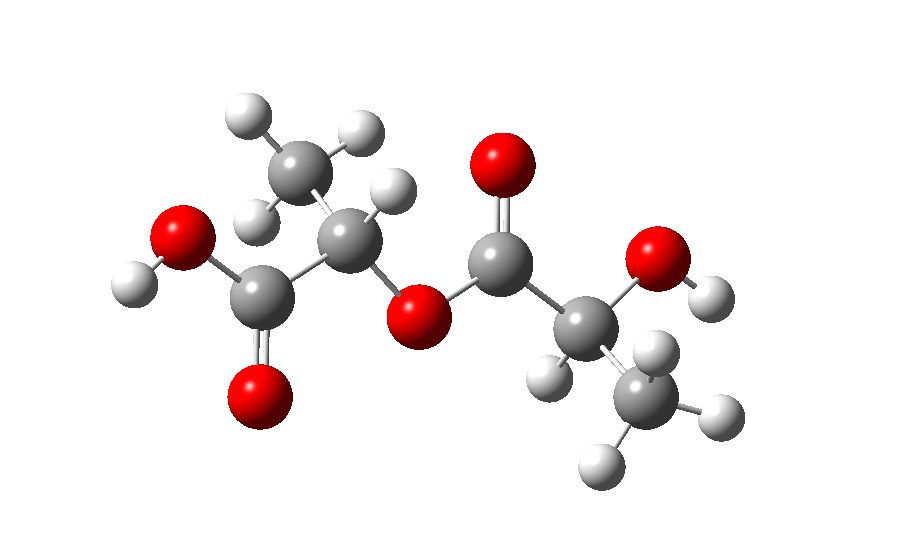
\includegraphics[width=1.2\linewidth]{img/pla_1d.png}
    	\end{subfigure}
    	\begin{subfigure}{0.33\textwidth}
    		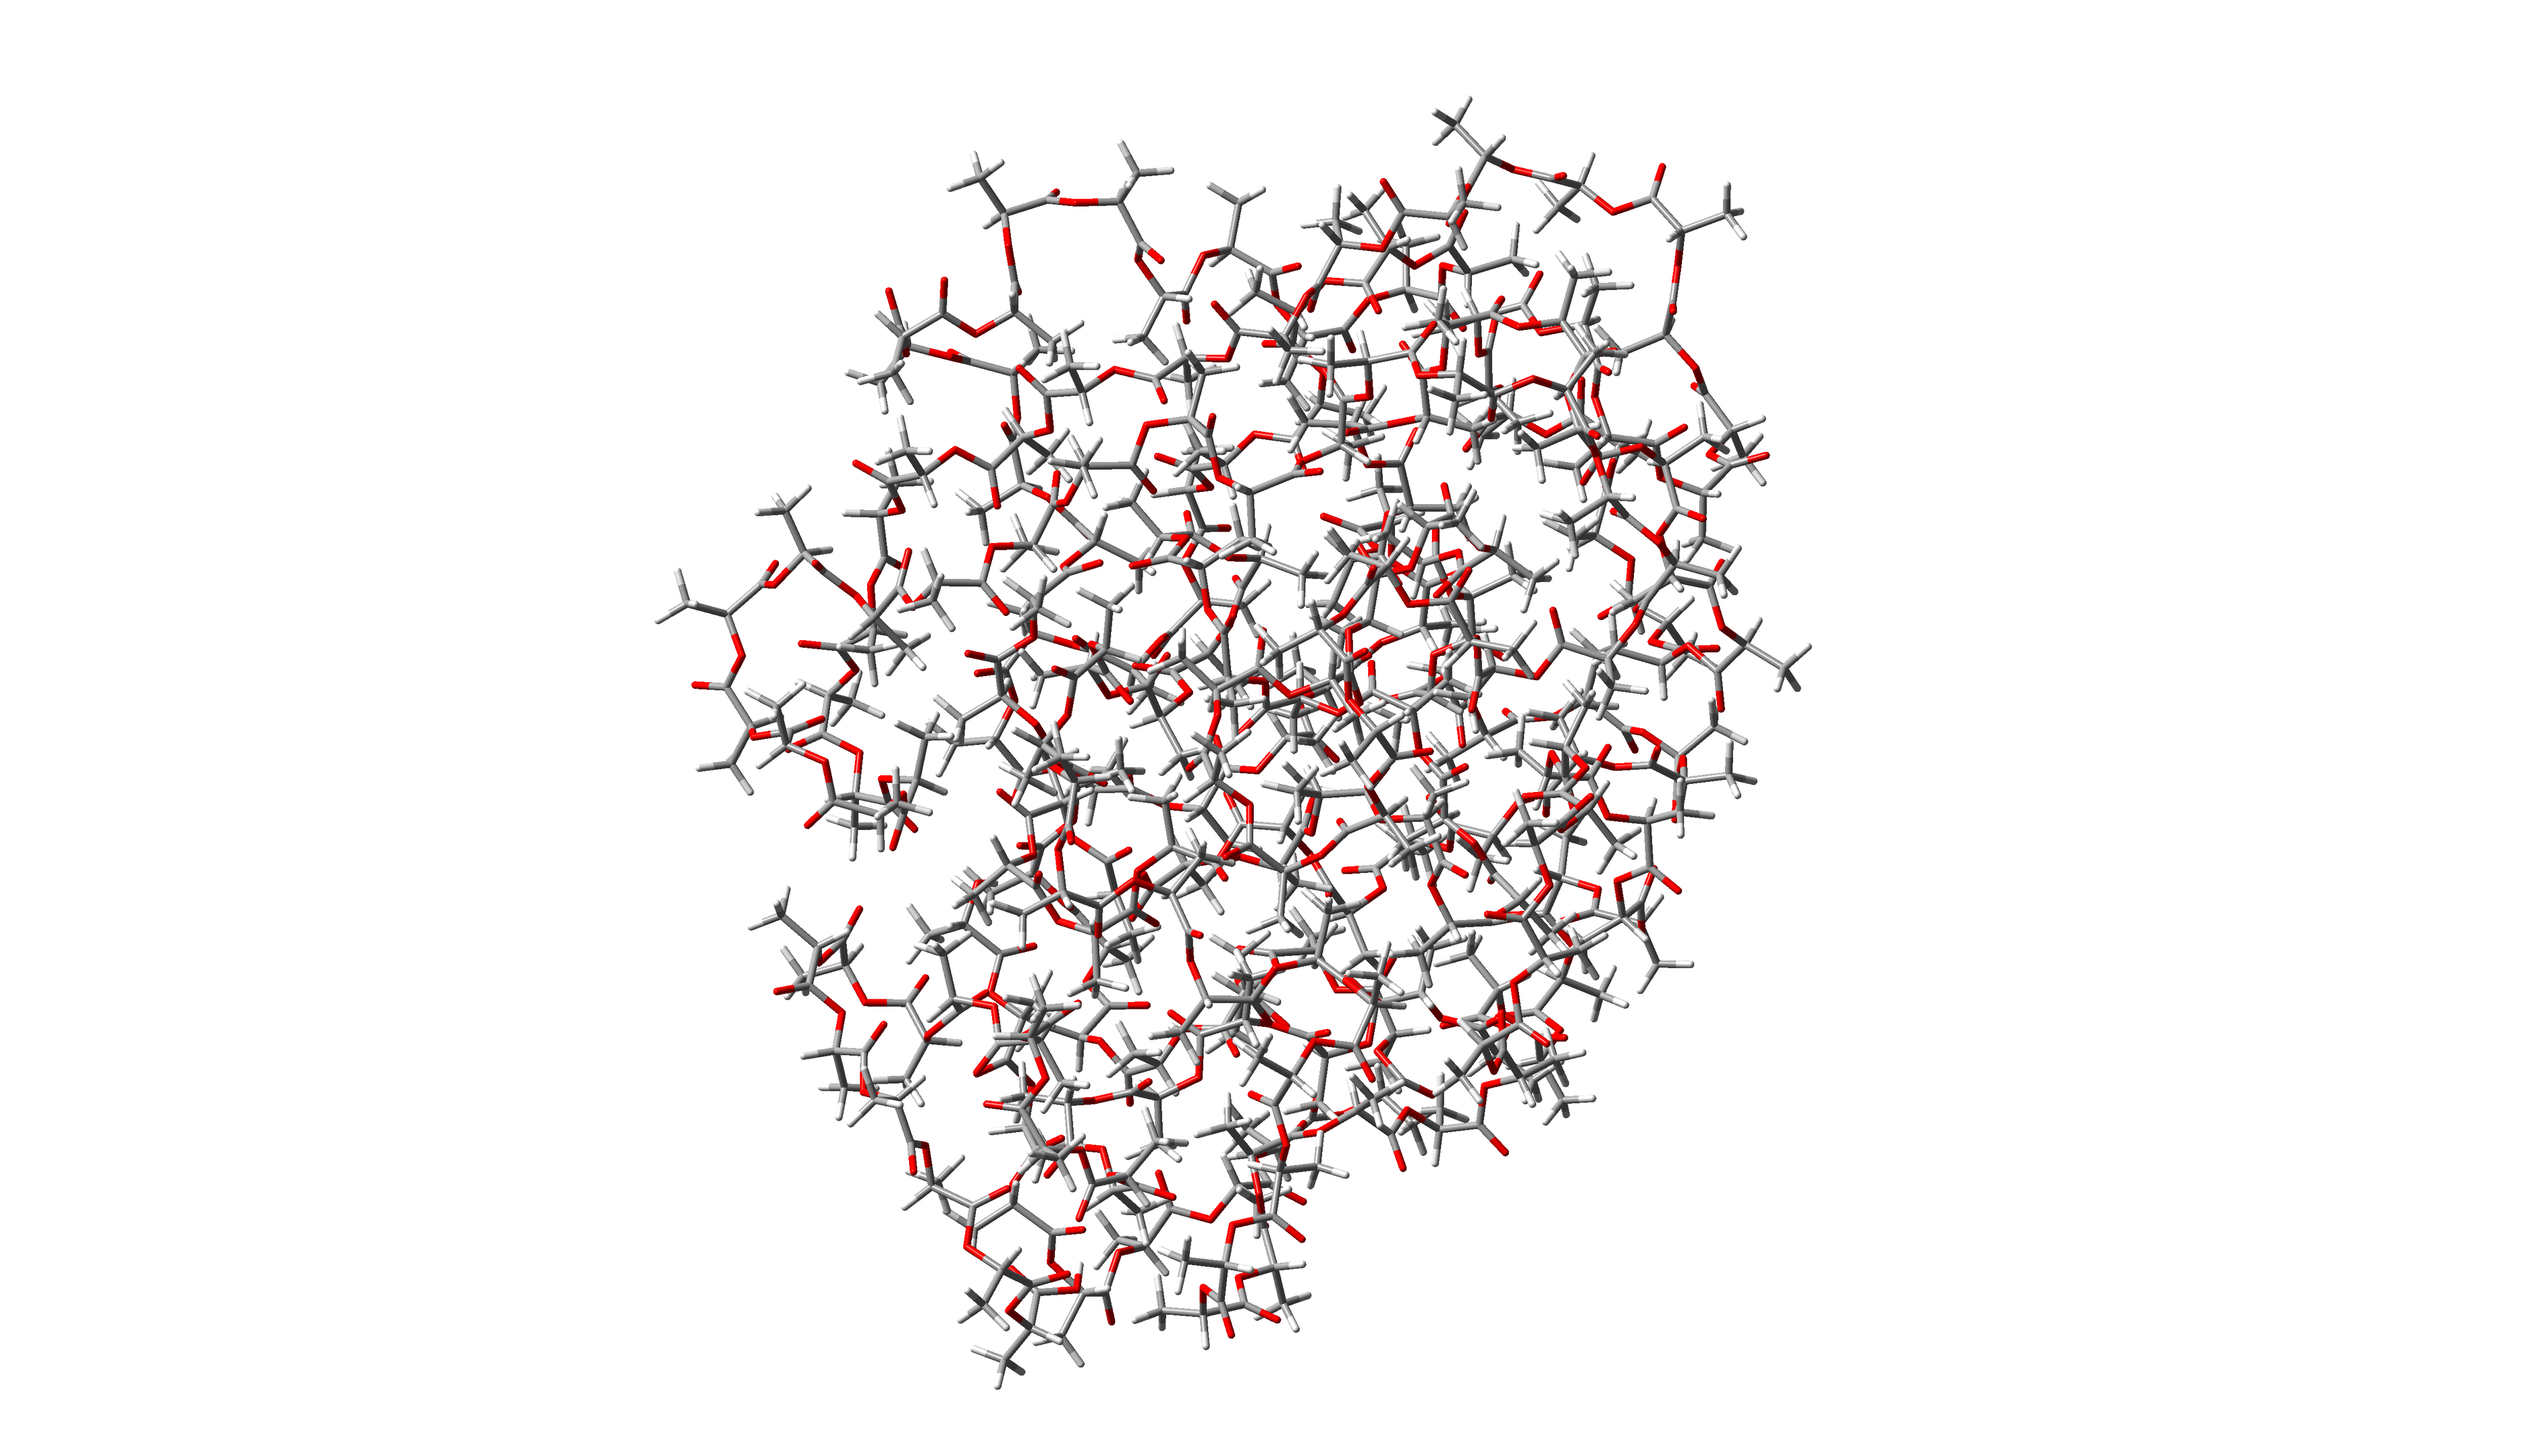
\includegraphics[width=1.4\linewidth]{img/pla_100g_tube.png}
    	\end{subfigure}
    	\caption{PLA formula on the left, PLA dimer block representing the chain unit used to build up polymer chain in the middle and a PLA chain containing 100 dimer block used to create mixtures with APIs on the right.}
    	\vspace{-0.5cm}
    	\label{fig:pla}
    \end{figure}
    
    \subsection{Active pharmaceutical ingredients}

   % \subsubsection{Ibuprofen}

    %\subsubsection{Naproxen}
    The second selected API is \textbf{naproxen} a non-steroidal anti-inflammatory drug, used as a painkiller. Naproxen contains three oxygen atoms (one carboxyl group and one ether bond), the structure is shown in Figure \ref{fig:APIs} on the right. According to its structure, naproxen can donate one hydrogen bond and accept up to three hydrogen bonds. Naproxen is a white crystalline powder, with a molar weight of $M_\mathrm{w}$~=~230.263~$\mathrm{g\ mol^{-1}}$ and melting point 429.3 K \cite{stejfa_heat_2021}.

    %\subsubsection{Carbamazepine}
    \textbf{Carbamazepine} is a representative anticonvulsant, which is used for the treatment of seizures and neuropathic pain. Carbamazepine contains two nitrogen atoms (amide group) and one oxygen in the carboxyl group; its structure is shown in Figure \ref{fig:APIs} on the left side. According to its structure, carbamazepine can accept and donate one hydrogen bond. Carbamazepine is a white crystalline powder, with a molar weight of $M_\mathrm{w}$~=~236.273~$\mathrm{g\ mol^{-1}}$ and melting temperature of 463.6 K \cite{stejfa_heat_2021}.

    %\subsubsection{Indomethacine}
	\begin{figure}[htb!]
		%\centering
		\hspace{1.2cm}
		\subfloat{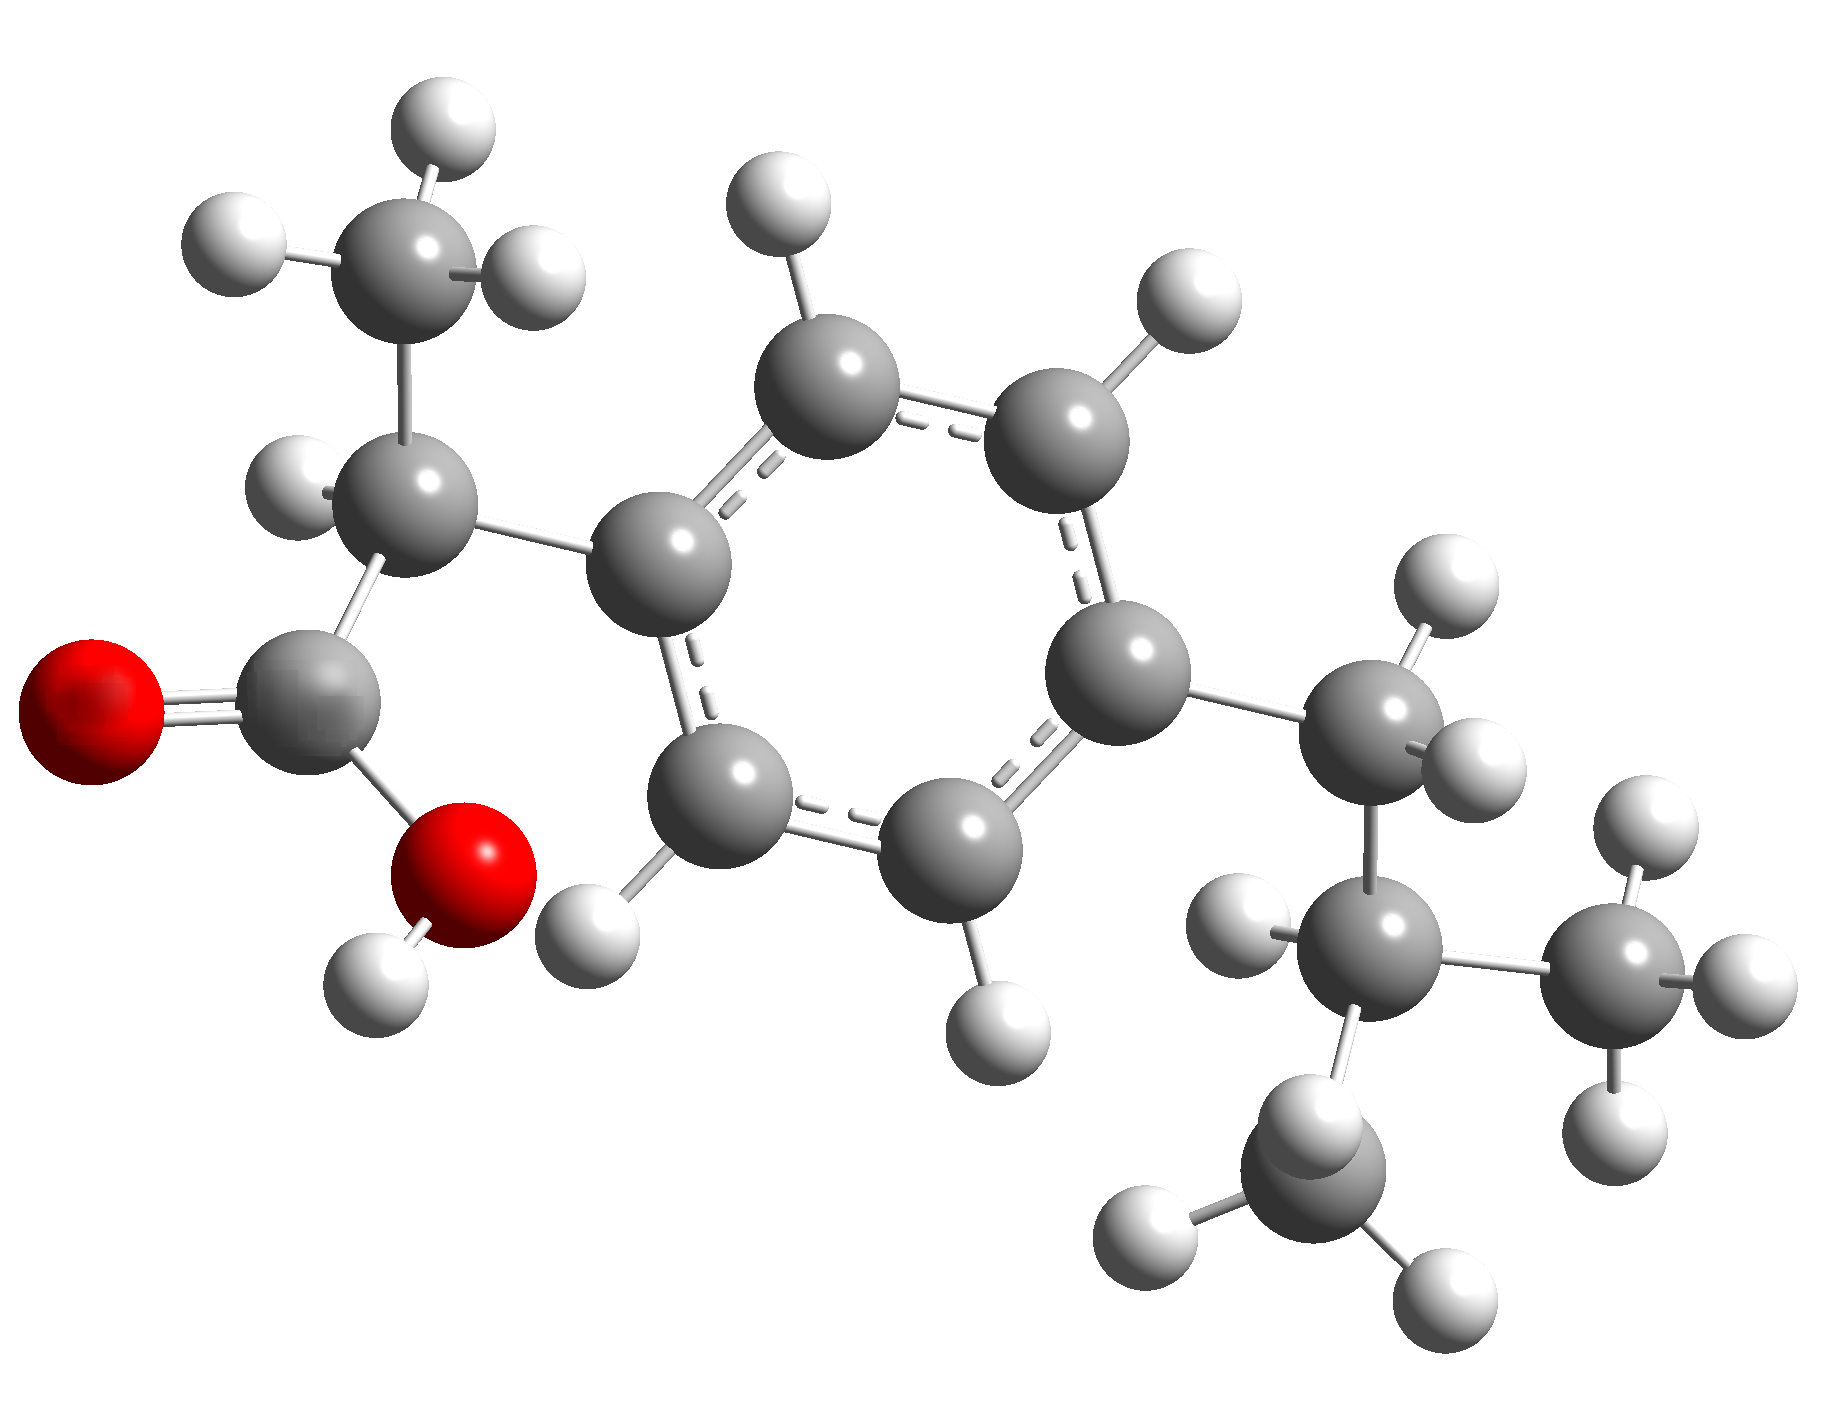
\includegraphics[width=0.35\linewidth]{img/ibu_s.png}}
		\hspace{2cm}
		\subfloat{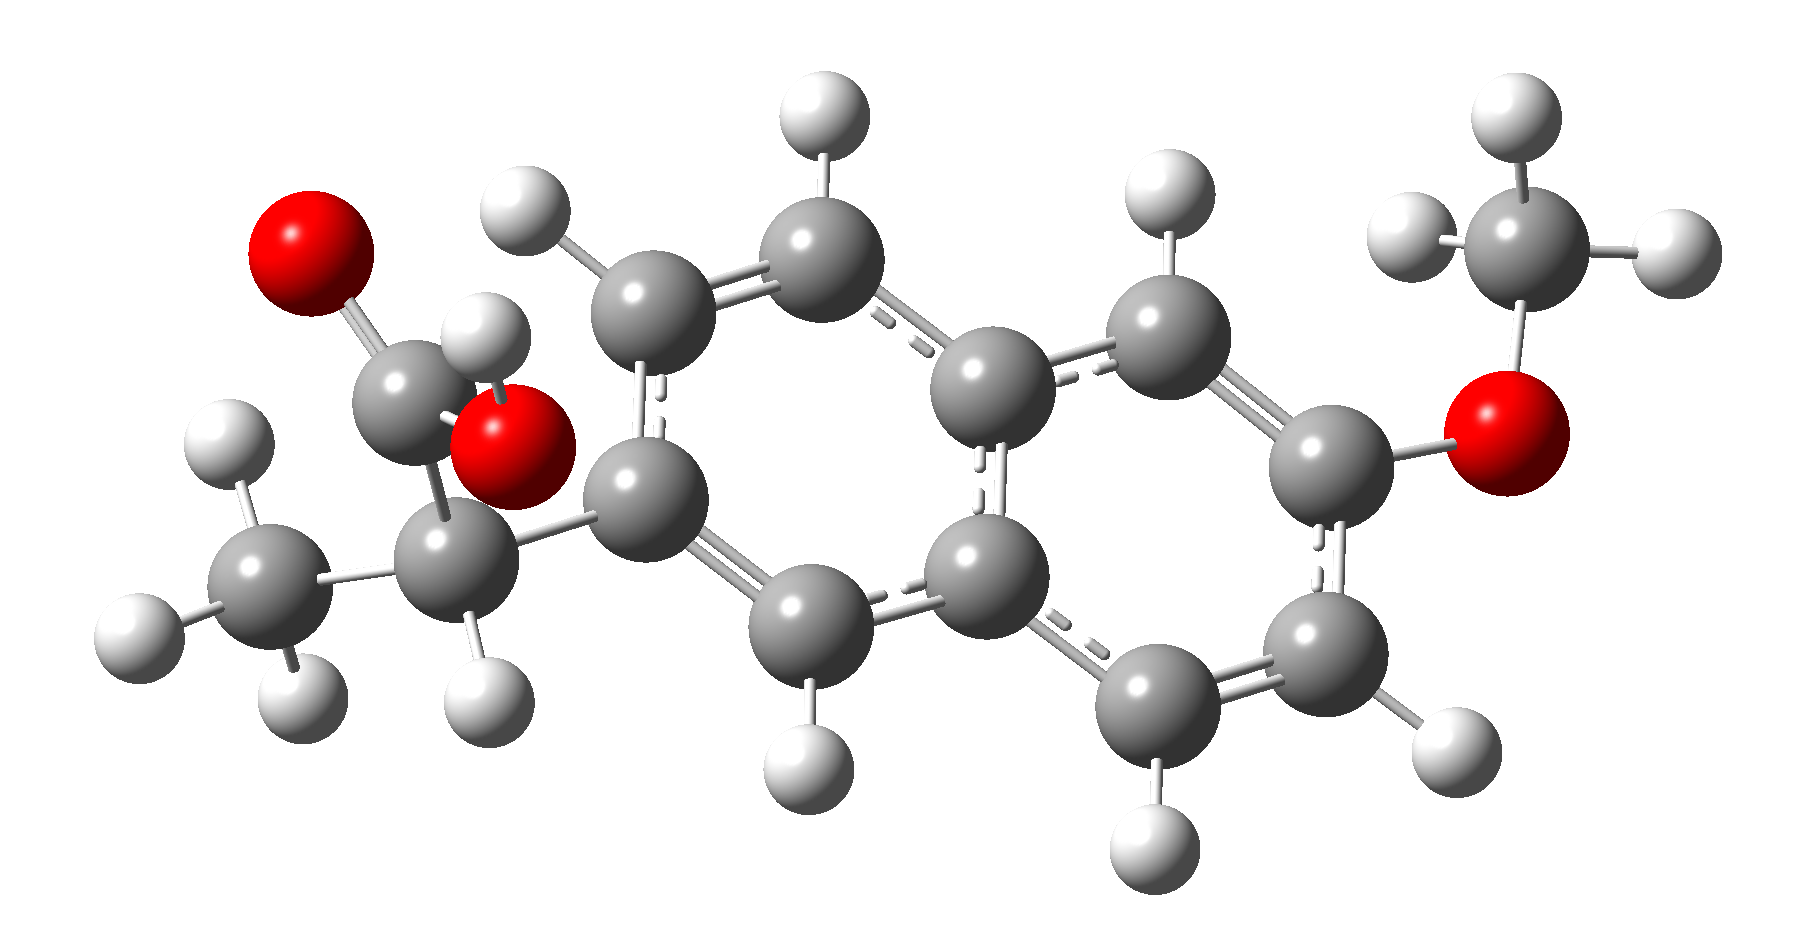
\includegraphics[width=0.45\linewidth]{img/nap.png}}\\
		\subfloat{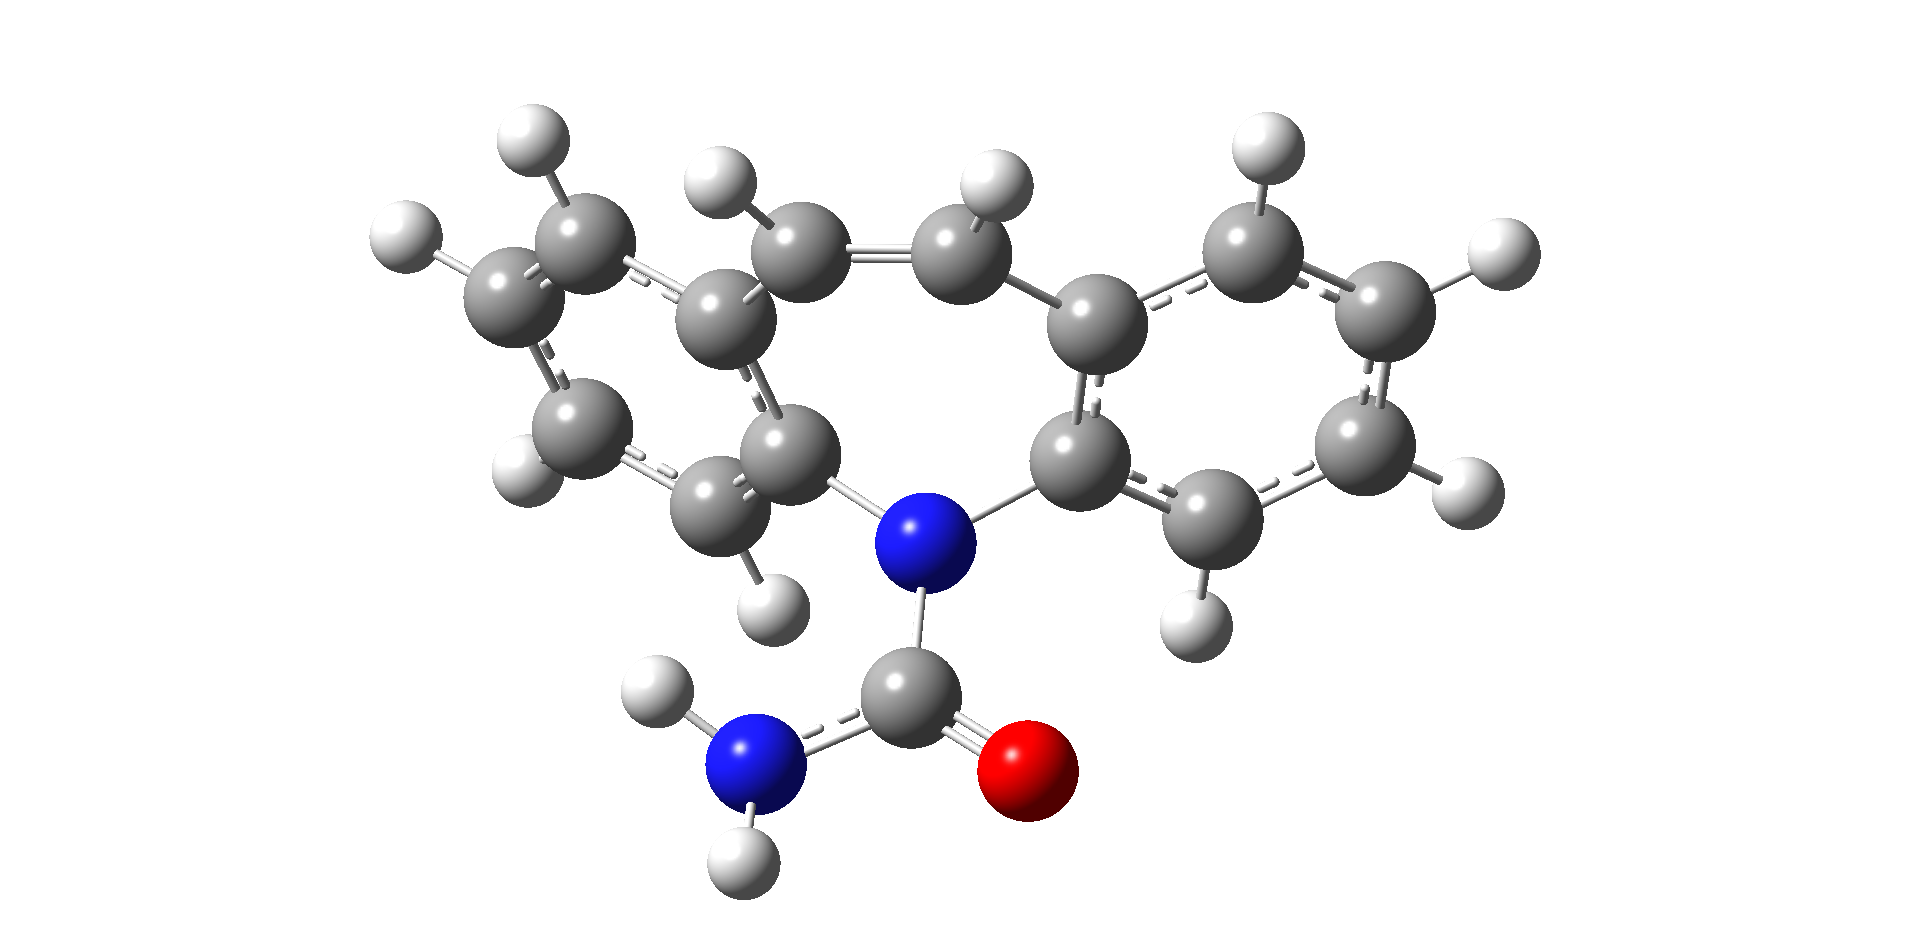
\includegraphics[width=0.6\linewidth]{img/cbz_svk.png}}
		\subfloat{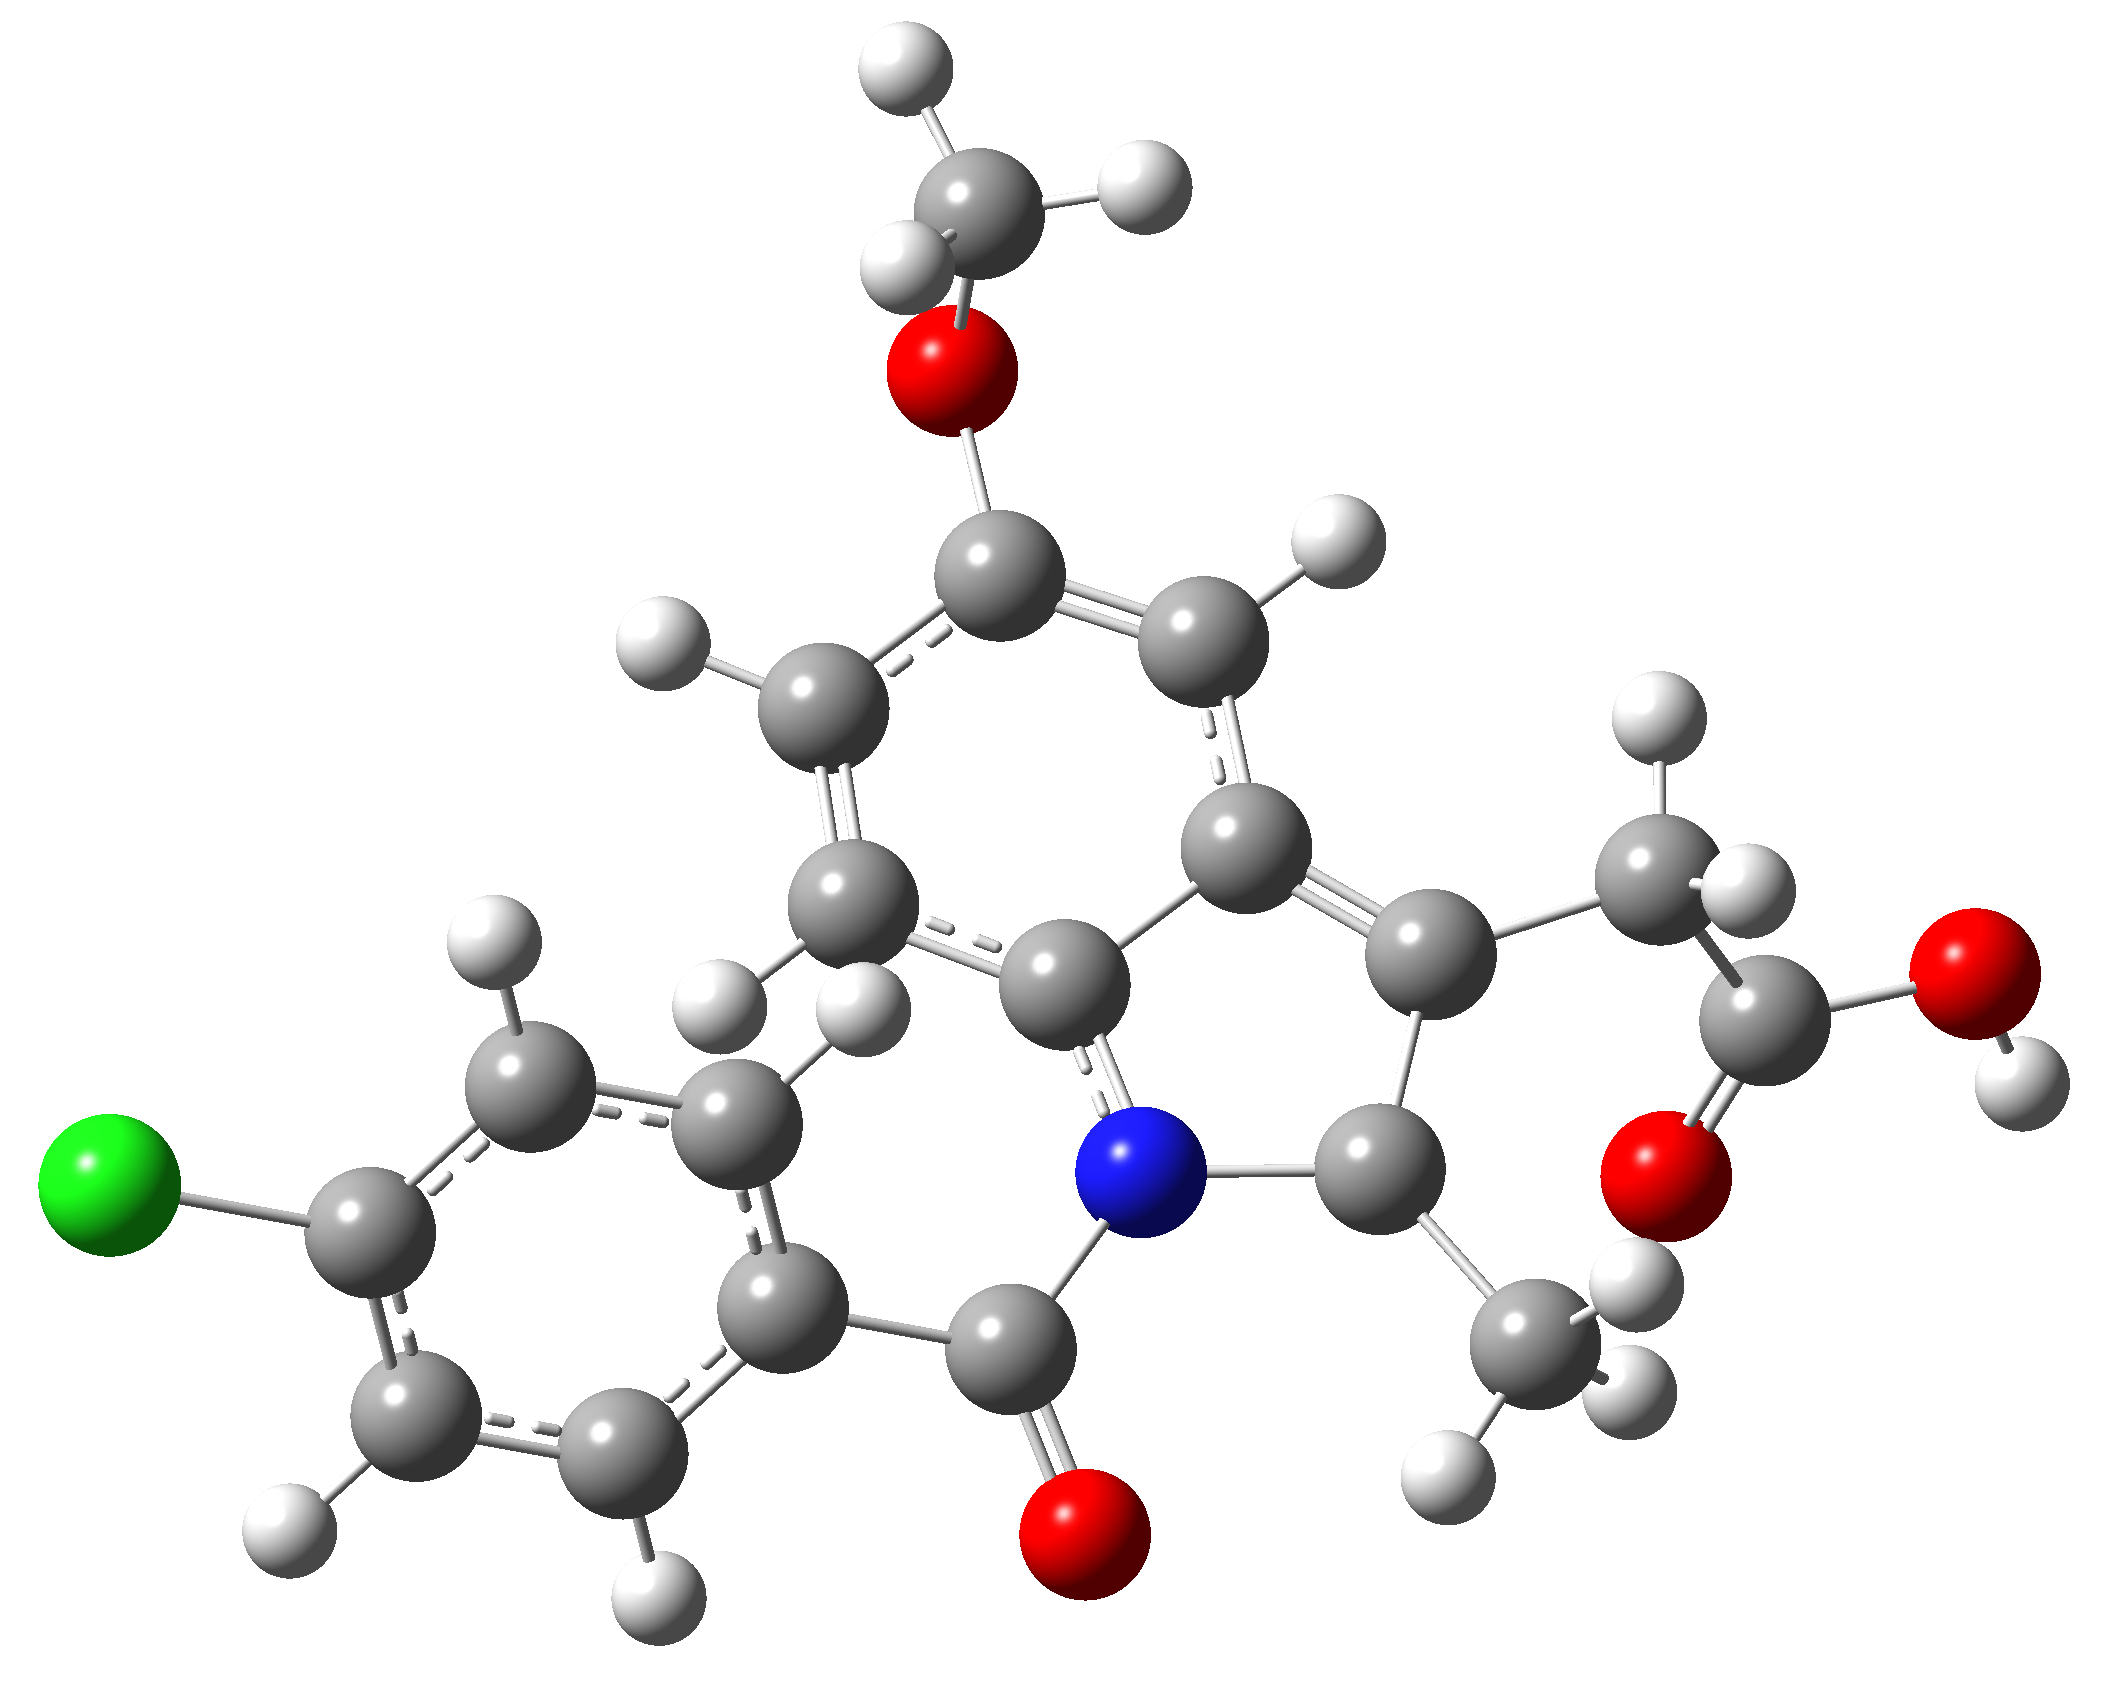
\includegraphics[width=0.4\linewidth]{img/indo.png}}
		\vspace{-0.5cm}
		\caption{Molecular structures of ibuprofen (\textbf{top left}), naproxen (\textbf{top right}), carbamazepine (\textbf{bottom left}) and indomethacin (\textbf{bottom right}).}
		\label{fig:APIs}
	\end{figure}

    %\subsubsection{Sulfathiazole}
    The selected API was \textbf{sulfathiazole} as a representative antibiotic drug from the sulfonamides group, which is used in the treatment of pyogenic cutaneous infections \cite{sulfathiazole_usage}. Sulfathiazole is a white crystalline powder, with molar weight $(M_\mathrm{w})$ =255.3 $\mathrm{gmol^{-1}}$ \cite{sulfathiazole}, which is highly polymorphic, there are 5 polymorphs discovered so far \cite{caron}. All known polymorphs of sulfathiazole crystallize in the $P2_1/c$ space group, but there are differences in intermolecular bonding and structural properties \cite{sulfathiazole_exp}. For our research, we chose the II polymorph, the structure of which is pictured in Figure \ref{fig:sulfathiazole}, there are four molecules of sulfathiazole in the crystal monoclinic unit cell. Our goal is to use quantum computing methods to determine the charges on atoms to complete the force field file model, and then to use MD to validate the model through comparison of simulated crystallographic parameters and density with experimental data.

    \begin{figure}[htb!]
	\begin{subfigure}{0.5\textwidth}
		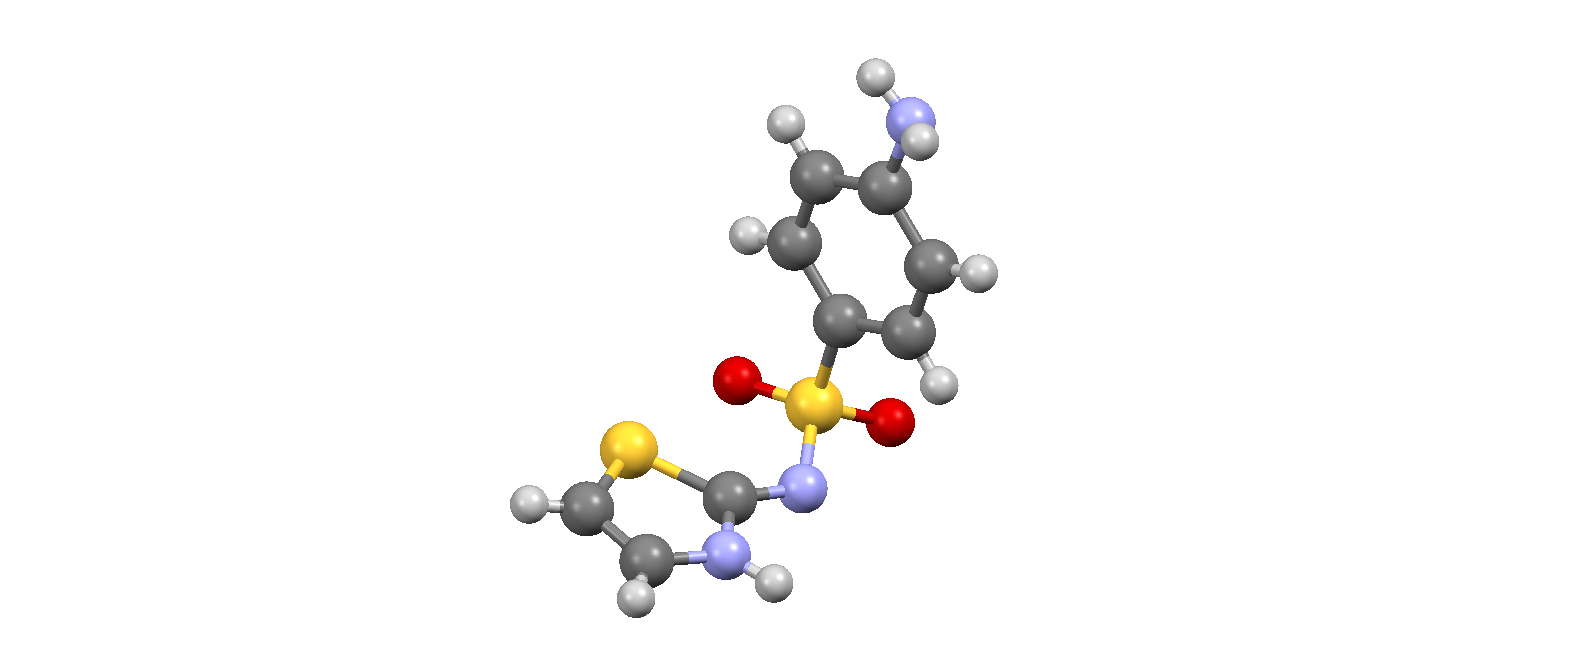
\includegraphics[width=1.2\linewidth]{img/sulfathiazol.png} 
	\end{subfigure}
	\begin{subfigure}{0.5\textwidth}
		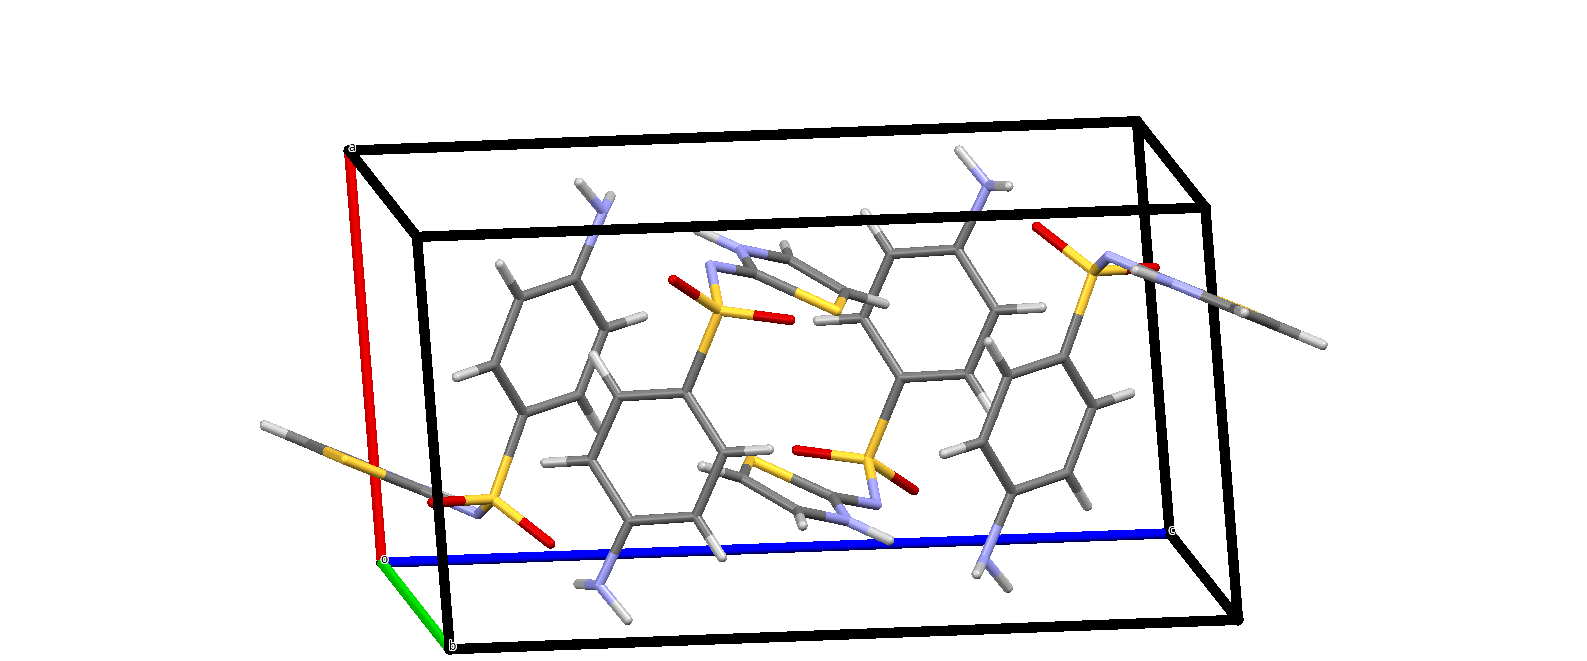
\includegraphics[width=1.1\linewidth]{img/sulfathiazol_packing.png}
	\end{subfigure}
	\caption{Sulfathiazole - molecular structure on the left and a unit cell of its II polymorph on the right.}
	\label{fig:sulfathiazole}
\end{figure}
